\chapter{Literaturrecherche}
\label{sec:literature_review}

Die Grundlage für das weitere Vorgehen bildet eine Literaturrecherche. Das Ziel dabei ist es, einen Überblick über bereits evaluierte Erklärungstypen in verschiedenen Kontexten zu erhalten. Aus den Typen sowie unterschiedlichen Evaluationsarten kann dann der zu entstehende Leitfaden abgeleitet werden.

Die Literaturrecherche besteht aus einer Planungs- und einer Durchführungsphase. In der Planungsphase wurden die Rahmenbedingungen dafür festgelegt, welche vorangegangen Arbeiten für das Ableiten eines Leitfadens zur Integration von Erklärungen geeignet sind. Anschließend werden in der Durchführungsphase alle daraus resultierenden Veröffentlichungen weiter gefiltert und für den Leitfaden zur Integration von Erklärungen wichtigen Informationen extrahiert.

\section{Planung}

Als Methode für die Literaturrecherche ist die Suchstring-Methode zur Anwendung gekommen. Dabei werden am Anfang die Datenbanken und Suchbegriffe definiert, um eine initiale Menge an Suchergebnissen zu erhalten.

Als Datenbanken wurden für die Suche \textit{ACM Digital Libraray}\footnote{https://dl.acm.org}, \textit{IEEE Xplore}\footnote{https://ieeexplore.ieee.org}, \textit{Science Direct}\footnote{https://www.sciencedirect.com} sowie \textit{Springer Link}\footnote{https://link.springer.com} verwendet. Die genannten Datenbanken wurden gewählt, da sie bereits für Literaturrecherchen im Bereich von Erklärbarkeit eingesetzt wurden \cite{nunes_systematic_2017, carvalho2017quality}. Bei der Such in \textit{Science Direct} und \textit{Springer Link} wurden die Ergebnisse auf den Bereich \textit{Computer Science} beschränkt. Weitere Filtereinstellungen für jede Datenbank sind in \autoref{sec:appendix_search_filter} zu finden.

Als Zeitraum für die Veröffentlichungen wurde das Jahr 2015 bis zur Durchführung der Suche (08.06.21) gewählt. 2015 wurde dabei als Startjahr gewählt, da zu diesem Zeitpunkt die Zahl der Veröffentlichungen zum Thema Erklärbarkeit mit Fokus auf die Wahrnehmung von Nutzern deutlich ansteigt und eine zusätzliche Betrachtung der ersten Phase von Veröffentlichungen zu Erklärbarkeit mit Blick auf Psychologie um 1990 den Rahmen dieser Arbeit überschreiten würde.

\subsection{Definition der Suchbegriffe}

Bei der Definition der Suchbegriffe wurden zunächst Schlüsselbegriffe definiert. Eine vollständige Übersicht ist in \autoref{tab:search_terms} zu sehen. Dabei wurden drei Blöcke von Begriffen identifiziert. Zur Themenabgrenzung muss jedes Suchergebnis ein Synonym für\glqq Erklärung\grqq{} oder \glqq Erklärbarkeit\grqq{} aufweisen. Da diese Arbeite unter anderem Einflüsse bzw. Evaluationen untersucht, besteht der zweite Begriffsblock aus solchen der Wortfamilie \glqq Evaluation\grqq{}. Aus der Betrachtung von externer Qualität wurden als letzter Block Begriffe, welche mit dem Gebiet der Mensch-Maschine Kommunikation in Verbindung stehen gewählt. Der Suchstring wie im Folgenden dargestellt ist dabei so aufgebaut, dass zusätzlich zur ersten Bedingung entweder ein Begriff aus dem zweiten oder dritten Block von Begriffen auf ein Suchergebnis zutreffen muss.

\bigskip

\noindent Suchstring: \textbf{((explainability OR explanation OR explanations OR explainable) AND (evaluation OR assessment OR analysis OR impact OR HCI OR \glqq human-computer interaction\grqq{} OR \glqq human-computer interfaces \grqq{} OR interaction OR \glqq user interface\grqq{} OR usability))}

\bigskip

Zur Kontrolle, ob die Suche relevante Ergebnisse liefert wurden view bekannte Arbeiten verwendet, von denen bekannt war, dass diese Antworten auf die Forschungsfragen enthalten: \citeauthor{chazette_end-users_nodate} \cite{chazette_end-users_nodate}, \citeauthor{chazette2020explainability} \cite{chazette2020explainability}, \citeauthor{kohl_explainability_2019} \cite{kohl_explainability_2019}, \citeauthor{sokol_explainability_2020} \cite{sokol_explainability_2020}.

\begin{table}[htb!]
    \begin{tabular}{p{.24\textwidth}p{.24\textwidth}p{.43\textwidth}}
        \hline
        Erklärbarkeit  & Evaluation & Mensch-Maschine Kommunikation             \\
        \toprule
        explainability          & evaluation    & HCI                           \\
        explanation             & assessment    & human-computer interaction    \\
        explanations            & analysis      & human-computer interfaces     \\
        explainable             & impact        & interaction                   \\
                                &               & user interface                \\
                                &               & usability                     \\              
        \toprule
    \end{tabular}
\caption{Schlüsselbegriffe für die Konstruktion des Suchstrings}
\label{tab:search_terms}
\end{table}

\subsection{Auswahlkriterien für Primärliteratur}

Um Suchergebnisse auf die für das Ziel der dieser Arbeit zu verwendenden Ergebnisse zu begrenzen wurden Bedingungen für das Selektieren (\textit{Inclusion Criteria: IC}) und ausschließen (\textit{Exculsion Criteria: EC}) gewält:

\subsubsection{Bedingungen}

\begin{enumerate}
    \item[IC1] Die Arbeit muss ein \textit{Peer Review} haben.
    \item[IC2] Die Arbeit muss in Englisch oder Deutsch verfasst sein.
    \item[IC3] Die Arbeit muss entweder die Evaluation einer bestimmten Erklärung oder einen Überblick über verschiedene Evaluationsmöglichkeiten enthalten.
    \item[IC4] Die Arbeit muss End-Nutzer von erklärbaren Systemen als Stakeholder von Erklärungen in Betracht ziehen.
\end{enumerate}

\subsubsection{Ausschlüsse}

\begin{enumerate}
    \item[EC1] Die Arbeit darf sich nicht ausschließlich darauf fokussieren, wie Erklärungen automatisch generiert werden können (Algorithmus-Evaluation).
    \item[EC2] Die Arbeit darf sich nicht ausschließlich auf das Verstehen von zugrundeliegenden Algorithmen beschränken (ML-\textit{Interpretability} ).
\end{enumerate}


\section{Durchführung}

% wichtige zitierte wie \cite{nunes_systematic_2017} wurden trotzdem genommen.

Nach der initialen Suche wurden mehrere Filterschritte durchgeführt. \autoref{fig:04_literature_review_selection_process} bietet einen Überblick über das Auswahlverfahren der Arbeiten, auf denen die hier entstandenen Ergebnisse aufbauen. Der Auswahlprozess ist in drei Iterationen erfolgt. Die Suche in den vier vorgestellten Datenbanken hat insgesamt 790 Ergebnisse ergeben. Dabei gab es 141 Duplikate. Die initiale Menge nach der Suche enthielt folglich 649 wissenschaftliche Arbeiten. Da die Suche auf die genannten vier Datenbanken beschränkt und passende Filter genutzt wurden, erfüllen diese Veröffentlichungen bereits die Kriterien des \textit{Peer Reviews}([IC1]).

\begin{figure}[htb]
    \centering
    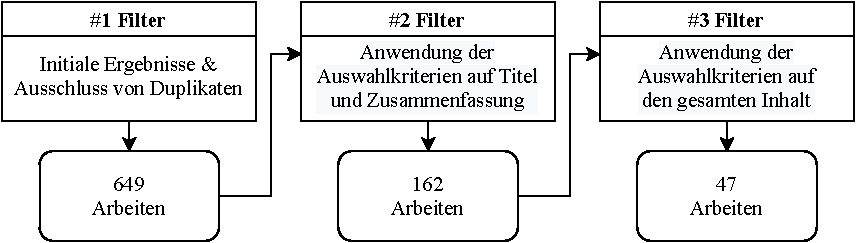
\includegraphics[width=\textwidth]{contents/04_literature_review/res/selection_process.pdf}
    \caption{Auswahlverfahren der Literaturrecherche}
    \label{fig:04_literature_review_selection_process}
\end{figure}

In einem zweiten Schritt wurden die Selektionskriterien auf den Titel und die Zusammenfassung der Arbeiten angewendet. Für die übrigen 162 Veröffentlichungen wurde der Volltext auf die Kriterien überprüft, wobei am Ende 47 Arbeiten alle Selektionskriterien erfüllt haben. Im Anschluss an die Auswahl wurden neun weitere Ergebnisse aufgenommen, die zum Verständnis einer anderen Arbeit wichtig waren und ebenfalls die Selektionskriterien erfüllt haben. Final enthält die Menge der wissenschaftlichen Arbeiten, die als Informationsgrundlage für die Erstellung eines Leitfadens zur Integration von Erklärungen gedient hat, 56 Arbeiten.

\pagebreak

\section{Ergebnisse}
%Paper Typen, die am Ende herauskamen:

%Die Paper können in Zwei Kategorien eingeteilt werden: Paper, die 

\begin{table}
    \begin{center}
        \begin{tabular}{p{.3\textwidth}p{.3\textwidth}p{.31\textwidth}}
            \hline
             & Empirische Strategie & Quellen \\
             \toprule
             Evaluation &  & \\
            Qualitätsaspekte                                                                &
            Kontrolliertes Experiment                                                       &
                 \cite{tintarev_designing_nodate} \cite{sato_context_nodate} \cite{eiband_impact_2019} \cite{tsai_evaluating_2019} \cite{hernandez-bocanegra_effects_2020} \cite{balog_measuring_2020} \cite{kunkel_let_2019} \cite{schaffer_i_2019} \cite{weitz_you_2019} \cite{yamada_evaluating_2016} \cite{sato_action-triggering_2019} \cite{haspiel_explanations_2018} \cite{zahedi_towards_2019} \cite{zolotas_towards_2019} \cite{riveiro_thats_2021}  \cite{martin_evaluating_2021} \cite{tsai_effects_2020}    \cite{neerincx_using_2018} \cite{schrills_color_2020} \cite{wang_is_2018} \cite{zhu_effects_2020} \cite{koo_why_2015} \cite{koo_understanding_2016} \cite{cheng2019explaining}
                 \\
                                                                                            &
            Case Study                                                                      &
                 \cite{martin_developing_2019} \cite{ehsan_human-centered_2020}
                 \\
                                                                                            &
            Umfrage                                                                         &
                \cite{chazette_end-users_nodate} \cite{chazette2020explainability} \cite{sokol_one_2020}
            \\
            Nutzer-Präferenz                                                                &
            Kontrolliertes Experiment                                                       &
                \cite{kouki_user_2017} \cite{mucha_interfaces_2021} \cite{abdulrahman_belief-based_2019} \cite{waa_evaluating_2021} \cite{wiegand_id_2020} \cite{stange_effects_2021} \cite{kaptein_personalised_2017} \cite{wiegand2019drive} \cite{du2019look}
            \\
            \midrule
            Analyse &  & \\
            Überblick                                                                       &
            Literaturrecherche                                                              &
                \cite{chazette_knowledge_nodate} \cite{sokol_explainability_2020} \cite{tintarev2015explaining} \cite{kohl_explainability_2019} \cite{rosenfeld_explainability_2019} \cite{cassens_ambient_2019} \cite{cirqueira_scenario-based_2020} \cite{rjoob_towards_2021} \cite{thomson_knowledge--information_2020} \cite{chari_explanation_2020} \cite{nunes_systematic_2017} \cite{sovrano_modelling_2020} \cite{ribera2019can} \cite{gunning2019darpa} \cite{doshi2017towards} \cite{lim_2009_assessing} \cite{tintarev2007survey}
                \\
                                                                                            &
            Umfrage                                                                         &
                \cite{brennen_what_2020} 
            \\ \toprule
        \end{tabular}
    \end{center}
    \caption{Ergebnisse der Literaturrecherche nach Art der Publikation}
    \label{tab:results_paper_types}
\end{table}

\begin{table}
    \begin{center}
        \begin{tabular}{p{.3\textwidth}p{.64\textwidth}}
            \hline
            Kontext                   & Quellen \\
            \toprule
            Allgemein                           &
                \cite{chazette_end-users_nodate} \cite{chazette2020explainability} \cite{chazette_knowledge_nodate} \cite{eiband_impact_2019} \cite{kohl_explainability_2019} \cite{ribera2019can} \cite{lim_2009_assessing} \\
            \tablerowspacing
            Intelligente Systeme (z.B. XAI)      & 
                \cite{waa_evaluating_2021} \cite{mucha_interfaces_2021} \cite{sokol_explainability_2020}  \cite{abdulrahman_belief-based_2019} \cite{brennen_what_2020} \cite{schaffer_i_2019} \cite{weitz_you_2019} \cite{riveiro_thats_2021} \cite{martin_developing_2019} \cite{martin_evaluating_2021} \cite{rosenfeld_explainability_2019} \cite{cassens_ambient_2019} \cite{cirqueira_scenario-based_2020}  \cite{ehsan_human-centered_2020} \cite{rjoob_towards_2021} \cite{thomson_knowledge--information_2020} \cite{chari_explanation_2020} \cite{sokol_one_2020}  \cite{neerincx_using_2018} \cite{schrills_color_2020} \cite{sovrano_modelling_2020} \cite{gunning2019darpa} \cite{doshi2017towards} \cite{cheng2019explaining}\\
            \tablerowspacing
            Empfehlungssysteme                  & 
                \cite{tintarev_designing_nodate} \cite{sato_context_nodate} \cite{balog_measuring_2020}  \cite{kouki_user_2017} \cite{tsai_evaluating_2019} \cite{hernandez-bocanegra_effects_2020} \cite{kunkel_let_2019} \cite{tintarev2015explaining} \cite{sato_action-triggering_2019} \cite{tsai_effects_2020} \cite{nunes_systematic_2017} \cite{tintarev2007survey}
            \\
            \tablerowspacing
            Autonomes Fahren                    &
                \cite{wiegand_id_2020} \cite{haspiel_explanations_2018} \cite{koo_understanding_2016} \cite{koo_why_2015} \cite{wiegand2019drive} \cite{du2019look}
            \\
            \tablerowspacing
            Mensch-Roboter-Interaktion          &
                \cite{stange_effects_2021} \cite{kaptein_personalised_2017} \cite{zolotas_towards_2019} \cite{wang_is_2018} \cite{zhu_effects_2020}
            \\
            \tablerowspacing
            Domain-Specific                     &
                \cite{yamada_evaluating_2016} \cite{zahedi_towards_2019}
            \\
            \toprule
        \end{tabular}
    \end{center}
    \caption{Kontext innerhalb von Erklärbaren Systemen, der von den Arbeiten untersucht wurde}
    \label{tab:paer_explanation_contexts}
\end{table}

